\documentclass[12pt, titlepage]{article}

\usepackage[margin=1in]{geometry}
\usepackage[round]{natbib}
\usepackage{multirow}
\usepackage{booktabs}
\usepackage{tabularx}
\usepackage{graphicx}
\usepackage{float}
\usepackage{hyperref}
\hypersetup{
    colorlinks,
    citecolor=blue,
    filecolor=black,
    linkcolor=red,
    urlcolor=blue
}

%% Comments

\usepackage{color}

\newif\ifcomments\commentstrue %displays comments
%\newif\ifcomments\commentsfalse %so that comments do not display

\ifcomments
\newcommand{\authornote}[3]{\textcolor{#1}{[#3 ---#2]}}
\newcommand{\todo}[1]{\textcolor{red}{[TODO: #1]}}
\else
\newcommand{\authornote}[3]{}
\newcommand{\todo}[1]{}
\fi

\newcommand{\wss}[1]{\authornote{blue}{SS}{#1}} 
\newcommand{\plt}[1]{\authornote{magenta}{TPLT}{#1}} %For explanation of the template
\newcommand{\an}[1]{\authornote{cyan}{Author}{#1}}

%% Common Parts

\newcommand{\progname}{Software Engineering} % PUT YOUR PROGRAM NAME HERE
\newcommand{\authname}{Team 21, Alkalytics
\\ Sumanya Gulati - gulats10
\\ Kate Min - mink9
\\ Jennifer Ye - yej52
\\ Jason Tran - tranj78} % AUTHOR NAMES                  

\usepackage{hyperref}
    \hypersetup{colorlinks=true, linkcolor=blue, citecolor=blue, filecolor=blue,
                urlcolor=blue, unicode=false}
    \urlstyle{same}
                                


\newcounter{acnum}
\newcommand{\actheacnum}{AC\theacnum}
\newcommand{\acref}[1]{AC\ref{#1}}

\newcounter{ucnum}
\newcommand{\uctheucnum}{UC\theucnum}
\newcommand{\uref}[1]{UC\ref{#1}}

\newcounter{mnum}
\newcommand{\mthemnum}{M\themnum}
\newcommand{\mref}[1]{M\ref{#1}}

\begin{document}

\title{Module Guide for \progname{}} 
\author{\authname}
\date{\today}

\maketitle

\pagenumbering{roman}

\section{Revision History}

\begin{tabularx}{\textwidth}{p{3cm}p{2cm}X}
\toprule {\bf Date} & {\bf Version} & {\bf Notes}\\
\midrule
11 Janury 2025 & 1.0 & Added initial content for Rev 0.\\
\bottomrule
\end{tabularx}
\\
\newline \newline
\emph{\textbf{Note:}} Please note that our team has adapted and extended this
Module Guide document to include the contents of an MIS or other such document.
For this reason, only one design document has been submitted.
\newpage

\section{Reference Material}

This section records information for easy reference.

\subsection{Abbreviations and Acronyms}

\renewcommand{\arraystretch}{1.2}
\begin{tabular}{l l} 
  \toprule		
  \textbf{symbol} & \textbf{description}\\
  \midrule 
  AC & Anticipated Change\\
  API & Application Programming Interface\\
  CSV & Comma Separated Values\\
  DAG & Directed Acyclic Graph \\
  JSON & JavaScript Object Notation\\
  KPI & Key Performance Indicator\\
  M & Module \\
  MG & Module Guide \\
  MIS & Module Interface Specification\\
  OS & Operating System \\
  R & Requirement\\
  SC & Scientific Computing \\
  SRS & Software Requirements Specification\\
  \progname & Explanation of program name\\
  UC & Unlikely Change \\
  UI & User Interface\\
  XML & Extensible Markup Language\\
  \bottomrule
\end{tabular}\\

\subsection{Notation}

\newpage

\tableofcontents

\listoftables

\listoffigures

\newpage

\pagenumbering{arabic}

\section{Introduction}

\subsection{Summary}
Alkalytics is a project designed to provide a scalable data management and analysis
solution for ocean alkalinity research, in particular by streamlining the data 
organization, querying, and visualization processes. Through its various modules, 
the primary goal of the system is to offer a comprehensive solution for data 
ingestion, processing and reporting  while maintaining adaptability to future 
changes.\\
\newline
Each functional component is developed as an independent module to encapsulate 
specific responsibilities, minimize dependencies, and promote information
hiding. This modular approach, advocated for widely in the software sector, not only
simplifies development and testing but also allows the system to accommodate evolving
user requirements and technology upgrades.

\subsection{Purpose}
This Module Guide (MG) has been written to serve as a roadmap for the Alkalytics system,
detailing its structure, functionality, and the relationships between its components.
It provides clarity on how the system meets the requirements outlined in the 
\href{https://github.com/SumanyaG/Alkalytics/blob/main/docs/SRS/SRS.pdf}{Software Requirements Specification (SRS)}
and supports the following stakeholders:
\begin{itemize}
  \item \textbf{New Developers}: To understand the modular architecture and ensure
  consistent implementation.
  \item \textbf{Maintainers}: To efficiently identify, update, or rewrite modules as needed.
  \item \textbf{Designers}: To validate the system's feasibility, flexibility, and alignment
  with project goals. 
\end{itemize}

\section{Anticipated and Unlikely Changes} \label{SecChange}

This section identifies potential changes to the system and classifies them into
two categories: anticipated changes (AC) as listed in section \ref{SecAchange} and
unlikely changes (UC) as listed in section \ref{SecUchange}. AC represent decisions 
that have been encapsulated within specific modules to minimize the impact of 
modifications while UC are those that, while possible, are fixed at the system 
architecture stage to reduce complexity.

\subsection{Anticipated Changes} \label{SecAchange}

Anticipated changes are the source of the information that is to be hidden
inside the modules. Ideally, changing one of the anticipated changes will only
require changing the one module that hides the associated decision. These changes
are encapsulated within specific modules to ensure the system's adaptability.

\begin{description}
  \item[\refstepcounter{acnum} \actheacnum \label{acHardware}:] \textbf{Hardware Configuration} - 
  The software may need to run on a different hardware platform like a server or on a 
  cloud solution. Changes in hardware specifications will primarily affect the \ref{mHH} 
  Module, isolating their imoact.
  
  \item[\refstepcounter{acnum} \actheacnum \label{acProcessing}:] \textbf{Data Processing Algorithms} - 
  Changes in analytical techniques along with advances in the machine learning space would
  introduce the need for new statistical models. These changes would be encapsulated in the
  Data Processing Module.

  \item[\refstepcounter{acnum} \actheacnum \label{acUI}:] \textbf{User Interface (UI) Design} - 
  Changes in analytical techniques along with advances in the machine learning space would
  introduce the need for new statistical models. These changes would be encapsulated in the
  Data Processing Module.

  \item[\refstepcounter{acnum} \actheacnum \label{acInput}:] \textbf{Input Data Formats} - 
  Currently, the system is expected to process data from Comma Separated Values (CSV) files only.
  In the future, however, modifications may have to be made to accommodate different file 
  formats (such as JavaScript Object Notation (JSON), Extensible Markup Language (XML) etc)
  which will be handled by the Data Ingestion Module without impacting other parts of the system.

  \item[\refstepcounter{acnum} \actheacnum \label{acSource}:] \textbf{Data Source Integration} - 
  New data sources such as third-party application programming interfaces (APIs), Internet of Things
  (IoT) devices may have to be added in the future. The Data Integration Module will have to be 
  redesigned to handle the integration of these new sources.

  \item[\refstepcounter{acnum} \actheacnum \label{acStorage}:] \textbf{Scaling Data Volume} - 
  As the number of experiments increases, the system may need to handle increasing data volumes
  as usage grows. This is addressed by the Data Storage Module which has been designed to support
  database scalability strategies.

  \item[\refstepcounter{acnum} \actheacnum \label{acRoles}:] \textbf{User Roles and Permissions} - 
  Future requirements may demand the addition of new user roles or changes to existing permissions.
  The Administration Module is designed to encapsulate these changes.

  \item[\refstepcounter{acnum} \actheacnum \label{acSchema}:] \textbf{Input Schema} - 
  With an increase in the number of diverse experiments, the schema for the data inputs may have to
  changed to support the addition or removal of new parameters. This is handled by the Data Ingestion
  Module.

  \item[\refstepcounter{acnum} \actheacnum \label{acNotifs}:] \textbf{Notification Rules} - 
  The conditions of triggering alerts or notifications may evolve, including but not limited to
  additional thresholds or new types of anomalies. These are handled by the Notifications Module
  without affecting other parts of the system.
  
  \item[\refstepcounter{acnum} \actheacnum \label{acMetrics}:] \textbf{Analytical Metrics} - 
  New metrics or Key Performance Indicators (KPIs) might be requested by stakeholders. This would
  involve adapting requirements by introducing new calculations or processing pipelines by modifying
  the Data Processing Module.
  
\end{description}

\subsection{Unlikely Changes} \label{SecUchange}

Unlikely changes are those that are fixed early in the design to simplify the system
and reduce complexity. These changes, if necessary, would have a significant impact on
multiple modules.

\begin{description}
  \item[\refstepcounter{ucnum} \uctheucnum \label{ucIO}:] \textbf{Input/Output Devices} - 
  The system is designed to support file-based inputs. Changes can include additional input
  and/or output methods such as direct hardware interaction, would require substantial
  redesign across multiple modules.
  
  \item[\refstepcounter{ucnum} \uctheucnum \label{ucSysArch}:] \textbf{Core System Architecture} -
  The underlying architectural decisions, such as the use of modular decomposition and separation
  of concerns, are not expected to change. Altering these decisions would necessitate a complete overhaul
  of the system.
  
  \item[\refstepcounter{ucnum} \uctheucnum \label{ucComms}:] \textbf{Communication Protocols} -
  The communication methods between modules such as function calls, API interactions etc are fixed. 
  Switching to a different communication protocol would impact the interfaces of all interacting modules.

  \item[\refstepcounter{ucnum} \uctheucnum \label{ucLanguage}:] \textbf{Programming Language} -
  The choice of programming languages is asssumed to be fixed for the project. A change would
  require rewriting most of the system.

  \item[\refstepcounter{ucnum} \uctheucnum \label{ucDatabase}:] \textbf{Database Type} -
  The choice of storage solution (relational versus NoSQL databases, for example) is assumed to remain
  fixed. Switching to a different type of database would require reworking the Data Storage
  Module and parts of the Data Processing Module.

\end{description}

\section{Module Hierarchy} \label{SecMH}

This section provides an overview of the module design for the Alkalytics system.
The modules are summarized in a hierarchy that follows the principle of information
hiding. Each module encapsulates specific secrets, ensuring changes are localized
and do not affect unrelated parts of the system. These modules are summarized in
a hierarchy decomposed by secrets in table \ref{TblMH}. This hierarchy represented
as a directed acyclic graph, shown in \ref{FigMH}, shows relationships betweem
higher-level and lower-level modules, with the leaf modules representing those that
will actually be implemented.

\begin{description}
\item [\refstepcounter{mnum} \mthemnum \label{mHH}:] Hardware-Hiding Module
\item [\refstepcounter{mnum} \mthemnum \label{mBH}:] Behaviour-Hiding Module
\item [\refstepcounter{mnum} \mthemnum \label{mIN}:] Interface Module 
\item [\refstepcounter{mnum} \mthemnum \label{mAD}:] Administration Module 
\item [\refstepcounter{mnum} \mthemnum \label{mDA}:] Data Acquisition Module 
\item [\refstepcounter{mnum} \mthemnum \label{mDS}:] Data Storage Module 
\item [\refstepcounter{mnum} \mthemnum \label{mDR}:] Data Retrieval Module 
\item [\refstepcounter{mnum} \mthemnum \label{mINP}:] Input Module 
\item [\refstepcounter{mnum} \mthemnum \label{mPR}:] Processing Module 
\item [\refstepcounter{mnum} \mthemnum \label{mOU}:] Output Module 
\item [\refstepcounter{mnum} \mthemnum \label{mUID}:] UI Design Module
\item [\refstepcounter{mnum} \mthemnum \label{mVI}:] Visualization Module
\item [\refstepcounter{mnum} \mthemnum \label{mUM}:] User Management Module 
\item [\refstepcounter{mnum} \mthemnum \label{mCM}:] Configuration Management Module
\item [\refstepcounter{mnum} \mthemnum \label{mDI}:] Data Ingestion Module
\item [\refstepcounter{mnum} \mthemnum \label{mDV}:] Data Validation Module 
\item [\refstepcounter{mnum} \mthemnum \label{mDT}:] Data Transformation Module 
\item [\refstepcounter{mnum} \mthemnum \label{mML}:] Machine Learning Module
\item [\refstepcounter{mnum} \mthemnum \label{mRE}:] Reporting Module 
\item [\refstepcounter{mnum} \mthemnum \label{mNO}:] Notification Module
\end{description}

\begin{table}[h!]
\centering
\begin{tabular}{p{0.3\textwidth} p{0.3\textwidth} p{0.35\textwidth}}
\toprule
\textbf{Level 1} & \textbf{Level 2} & \textbf{Level 3}\\
\midrule

{Hardware-Hiding Module} & ~ & ~ \\
& Data Acquisition Module & \\
& Data Storage Module & \\
& Data Retrieval Module & \\
\midrule

{Behaviour-Hiding Module} & Input Module & Data Ingestion Module\\
& & Data Validation Module\\
& Processing Module & Data Transformation Module\\
& & Machine Learning Module\\
& Output Module & Reporting Module\\
& & Notifications Module\\
\midrule

{Interface Module} & UI Design Module & \\
& Visualization Module & \\
\midrule

{Administration Module} & User Management Module & \\
& Configuration Management Module & \\
\bottomrule

\end{tabular}
\caption{Module Hierarchy}
\label{TblMH}
\end{table}

\begin{figure}[htbp]
  \centering
  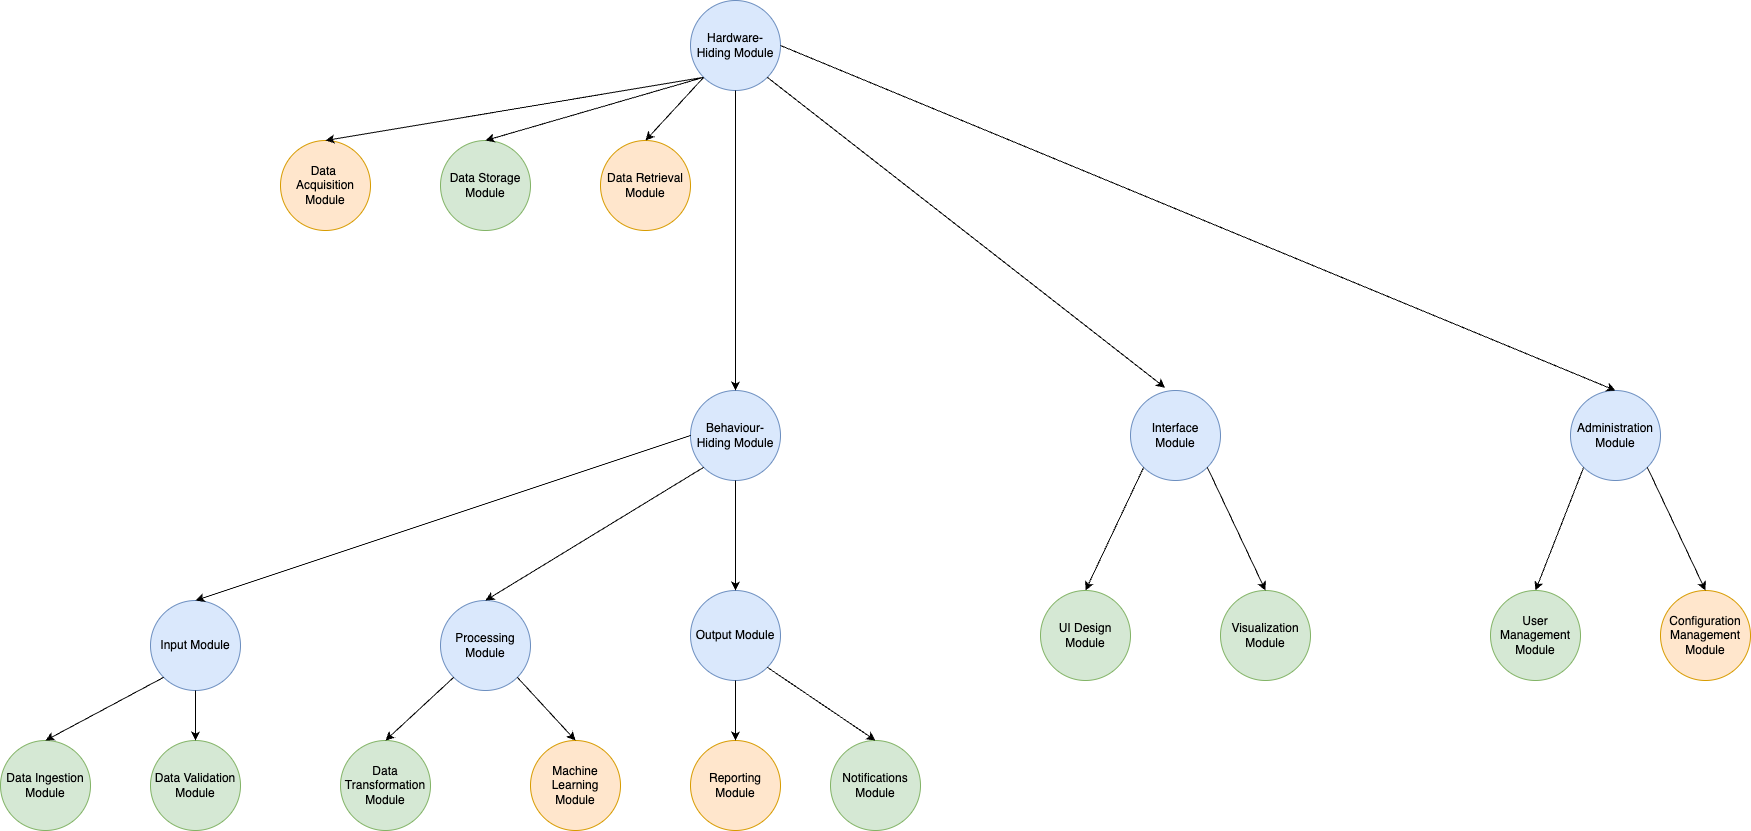
\includegraphics[width=\textwidth]{Diagrams/DAG.png}
  \caption{A DAG representing the implemented module hierarchy of Alkalytics.}
  \label{fig:FigMH}
\end{figure}

It must be noted that the blue nodes shown in figure \ref{fig:FigMH} represent 
`container' modules that act as high-level modules conatining leaf nodes that
can be implemented. The orange nodes represent modules that will not be implemented
for Revision 0 of Alkalytics and the green nodes represent modules that must be be implemented.

\section{Connection Between Requirements and Design} \label{SecConnection}

The design of the system is intended to satisfy the requirements developed in
the SRS. In this stage, the system is decomposed into modules. The connection
between requirements and modules is listed in Table~\ref{TblRT}.

\wss{The intention of this section is to document decisions that are made
  ``between'' the requirements and the design.  To satisfy some requirements,
  design decisions need to be made.  Rather than make these decisions implicit,
  they are explicitly recorded here.  For instance, if a program has security
  requirements, a specific design decision may be made to satisfy those
  requirements with a password.}

\section{Module Decomposition} \label{SecMD}

Modules are decomposed according to the principle of ``information hiding''
proposed by \citet{ParnasEtAl1984}. The \emph{Secrets} field in a module
decomposition is a brief statement of the design decision hidden by the
module. The \emph{Services} field specifies \emph{what} the module will do
without documenting \emph{how} to do it. For each module, a suggestion for the
implementing software is given under the \emph{Implemented By} title. If the
entry is \emph{OS}, this means that the module is provided by the operating
system or by standard programming language libraries.  \emph{\progname{}} means the
module will be implemented by the \progname{} software.

Only the leaf modules in the hierarchy have to be implemented. If a dash
(\emph{--}) is shown, this means that the module is not a leaf and will not have
to be implemented.

\subsection{Data Ingestion Modules (\mref{mDI})}

\begin{description}
\item[Secrets:]The data structure and algorithm used to implement the virtual
  hardware.
\item[Services:]Serves as a virtual hardware used by the rest of the
  system. This module provides the interface between the hardware and the
  software. So, the system can use it to display outputs or to accept inputs.
\item[Implemented By:] OS
\end{description}

\subsubsection{Uses}

\subsubsection{Syntax}
\begin{description}
  \item[Exported Constants] 
  \item[Exported Access Programs] 
\end{description}

\subsubsection{Semantics}
\begin{description}
  \item[State Variables]
  \item[Environment Variables]  
  \item[Assumptions] 
  \item[Access Routine Semantics] 
  \item[Local Function] 
\end{description}

\subsection{Data Processing Module}

\begin{description}
\item[Secrets:]The contents of the required behaviours.
\item[Services:]Includes programs that provide externally visible behaviour of
  the system as specified in the software requirements specification (SRS)
  documents. This module serves as a communication layer between the
  hardware-hiding module and the software decision module. The programs in this
  module will need to change if there are changes in the SRS.
\item[Implemented By:] --
\end{description}

\subsubsection{Data Storage Module (\mref{mInput})}

\begin{description}
\item[Secrets:]The format and structure of the input data.
\item[Services:]Converts the input data into the data structure used by the
  input parameters module.
\item[Implemented By:] [Your Program Name Here]
\item[Type of Module:] [Record, Library, Abstract Object, or Abstract Data Type]
  [Information to include for leaf modules in the decomposition by secrets tree.]
\end{description}

\subsubsection{Etc.}

\subsection{User Interface Module}

\subsection{Reporting Module}

\subsection{Notifications Module}

\subsection{Administration Module}

\begin{description}
\item[Secrets:] The design decision based on mathematical theorems, physical
  facts, or programming considerations. The secrets of this module are
  \emph{not} described in the SRS.
\item[Services:] Includes data structure and algorithms used in the system that
  do not provide direct interaction with the user. 
  % Changes in these modules are more likely to be motivated by a desire to
  % improve performance than by externally imposed changes.
\item[Implemented By:] --
\end{description}

\subsubsection{Etc.}

\section{MIS of Hardware-Hiding Module}
\subsection{Data Storage Module}

\section{MIS of Behaviour-Hiding Module}
\subsection{Data Ingestion Module}
\subsection{Data Validation Module}
\subsection{Data Transformation Module}
\subsection{Machine Learning Module}
\subsection{Reporting Module}
\subsection{Notifications Module}

\section{MIS of Interface Module}
\subsection{UI Design Module}
\subsection{Visualization Module}

\section{MIS of Administration Module}
\subsection{User Management Module}

\section{Traceability Matrix} \label{SecTM}

This section shows two traceability matrices: between the modules and the
requirements and between the modules and the anticipated changes.

% the table should use mref, the requirements should be named, use something
% like fref
\begin{table}[H]
\centering
\begin{tabular}{p{0.2\textwidth} p{0.6\textwidth}}
\toprule
\textbf{Req.} & \textbf{Modules}\\
\midrule
R1 & \mref{mHH}, \mref{mInput}, \mref{mParams}, \mref{mControl}\\
R2 & \mref{mInput}, \mref{mParams}\\
R3 & \mref{mVerify}\\
R4 & \mref{mOutput}, \mref{mControl}\\
R5 & \mref{mOutput}, \mref{mODEs}, \mref{mControl}, \mref{mSeqDS}, \mref{mSolver}, \mref{mPlot}\\
R6 & \mref{mOutput}, \mref{mODEs}, \mref{mControl}, \mref{mSeqDS}, \mref{mSolver}, \mref{mPlot}\\
R7 & \mref{mOutput}, \mref{mEnergy}, \mref{mControl}, \mref{mSeqDS}, \mref{mPlot}\\
R8 & \mref{mOutput}, \mref{mEnergy}, \mref{mControl}, \mref{mSeqDS}, \mref{mPlot}\\
R9 & \mref{mVerifyOut}\\
R10 & \mref{mOutput}, \mref{mODEs}, \mref{mControl}\\
R11 & \mref{mOutput}, \mref{mODEs}, \mref{mEnergy}, \mref{mControl}\\
\bottomrule
\end{tabular}
\caption{Trace Between Requirements and Modules}
\label{TblRT}
\end{table}

\begin{table}[H]
\centering
\begin{tabular}{p{0.2\textwidth} p{0.6\textwidth}}
\toprule
\textbf{AC} & \textbf{Modules}\\
\midrule
\acref{acHardware} & \mref{mHH}\\
\acref{acInput} & \mref{mInput}\\
\acref{acParams} & \mref{mParams}\\
\acref{acVerify} & \mref{mVerify}\\
\acref{acOutput} & \mref{mOutput}\\
\acref{acVerifyOut} & \mref{mVerifyOut}\\
\acref{acODEs} & \mref{mODEs}\\
\acref{acEnergy} & \mref{mEnergy}\\
\acref{acControl} & \mref{mControl}\\
\acref{acSeqDS} & \mref{mSeqDS}\\
\acref{acSolver} & \mref{mSolver}\\
\acref{acPlot} & \mref{mPlot}\\
\bottomrule
\end{tabular}
\caption{Trace Between Anticipated Changes and Modules}
\label{TblACT}
\end{table}

\section{Use Hierarchy Between Modules} \label{SecUse}

In this section, the uses hierarchy between modules is
provided. \citet{Parnas1978} said of two programs A and B that A {\em uses} B if
correct execution of B may be necessary for A to complete the task described in
its specification. That is, A {\em uses} B if there exist situations in which
the correct functioning of A depends upon the availability of a correct
implementation of B.  Figure \ref{FigUH} illustrates the use relation between
the modules. It can be seen that the graph is a directed acyclic graph
(DAG). Each level of the hierarchy offers a testable and usable subset of the
system, and modules in the higher level of the hierarchy are essentially simpler
because they use modules from the lower levels.

\wss{The uses relation is not a data flow diagram.  In the code there will often
be an import statement in module A when it directly uses module B.  Module B
provides the services that module A needs.  The code for module A needs to be
able to see these services (hence the import statement).  Since the uses
relation is transitive, there is a use relation without an import, but the
arrows in the diagram typically correspond to the presence of import statement.}

\wss{If module A uses module B, the arrow is directed from A to B.}

\begin{figure}[H]
\centering
%\includegraphics[width=0.7\textwidth]{UsesHierarchy.png}
\caption{Use hierarchy among modules}
\label{FigUH}
\end{figure}

%\section*{References}

\section{User Interfaces}

\wss{Design of user interface for software and hardware.  Attach an appendix if
needed. Drawings, Sketches, Figma}

\section{Timeline}

\wss{Schedule of tasks and who is responsible}

\wss{You can point to GitHub if this information is included there}

\bibliographystyle {plainnat}
\bibliography{../../../refs/References}

\newpage{}

\end{document}